% tlmgr install ...
\documentclass{article}
\usepackage{graphicx} % Required for inserting images
\usepackage{wrapfig}
\usepackage{amsmath} % Required for some math elements
\usepackage[margin=2cm]{geometry} % Set margins to 2cm
\usepackage[danish]{babel} % Set language to Danish
\usepackage{tocloft}
\usepackage{csquotes}
\usepackage{xcolor}
\usepackage{nicematrix}
\usepackage{caption}
% Required package
\usepackage{tikz}

% Input layer neurons' number
\newcommand{\inputnum}{3} 

% Hidden layer neurons' number
\newcommand{\hiddennum}{5}  

% Output layer neurons' number
\newcommand{\outputnum}{2} 

\usepackage[
  style=apa,
  sortcites=true,
  sorting=nyt,
  backend=biber,
  autocite=inline
]{biblatex}
\addbibresource{paper.bib}

\renewcommand\cftsecfont{\normalfont}
\renewcommand{\cftsecleader}{\cftdotfill{\cftsecdotsep}}
\renewcommand\cftsecdotsep{\cftdot}
\renewcommand\cftsubsecdotsep{\cftdot}
\renewcommand\cftsubsubsecdotsep{\cftdot}

\newcommand{\figureref}[1]{Figur \ref{#1}}


\makeatletter
\newcommand{\subject}[1]{\gdef\@subject{#1}}
\newcommand{\class}[1]{\gdef\@class{#1}}
\newcommand{\mentor}[1]{\gdef\@mentor{#1}}
\renewcommand{\maketitle}{\bgroup\setlength{\parindent}{0pt}
\begin{flushleft}
  \textbf{\@title}

  \@subject\\\vspace{1em}
  \@author\\
  \@class\\
  \@date\\\vspace{1em}
  Vejledere:\\\@mentor
\end{flushleft}\egroup
}
\makeatother

\title{\Huge{Studie Område Projekt}}
\subject{Matematik A / Programmering B}
\author{Victor Østergaard Nielsen}
\class{3di - H. C. Ørsted Gymnasiet Lyngby}
\date{15/12/2024}
\mentor{Jan Strauss Hansen (Matematik A) \\ Kristian Krabbe Møller (Programmering B)}

\begin{document}

\maketitle
\newpage

\tableofcontents
\newpage

\section{Opgaveformulering}
\textbf{Machine-learning}\\\\
\textbf{Hovedspørgsmål}: Hvordan kan et simpelt neuralt netværk, uden unødige abstraktioner eller biblioteker, anvendes tilgenkendelse af håndskrevne tal i realtid i et tegneprogram på computeren, og hvad er matematikken bag?\\\\
\textbf{Opgaveformulering}:\\
\begin{itemize}
  \item Redegør overordnet for begrebet neuralt netværk.
  \item Redegør for de grundlæggende matematiske principper bag neurale netværk herunder matriceregning.
  \item Redegør for valg af programmeringssprog ift. udvikling af programmer med neuralt netværk.
  \item Analysér hvordan et neutralt netværk kan programmeres, gerne uden unødvendige abstraktioner eller biblioteker, så det kan genkende håndskrevne tal i realtid i/fra et tegneprogram på computeren.
  \item Undersøg hvorledes programmet kan optimeres for at opnå lavest mulig fejlrate og evt. hvorledes støj i den analyserede data kan påvirke fejlraten.
  \item Diskuter og vurder hvorvidt neutrale netværk er den mest effektive tilgang til at genkende håndskrevne tal på en adaptiv og robust måde.
\end{itemize}

\newpage
\section{Indledning}


\newpage
\section{Matricer og matrixregning}
\subsection{Matricer}
En matrice er en tabel af tal, der er arrangeret i rækker og kolonner. En matrice kan repræsenteres med et stort bogstav, f.eks. $A$, og elementerne i matricen kan repræsenteres som $a_{ij}$, hvor $i$ er rækken og $j$ er kolonnen. En matrice med $m$ rækker og $n$ kolonner kaldes en $m \times n$ matrice. En matrice med lige mange rækker og kolonner kaldes en kvadratisk matrice. En matrice med kun én række kaldes en rækkevektor, og en matrice med kun én kolonne kaldes en søjlevektor. \parencite{Lauritzen_2019}\\\\
\begin{align}
  \underbrace{A = \begin{bmatrix}
    a_{11} & a_{12} & \ldots & a_{1n} \\
    a_{21} & a_{22} & \ldots & a_{2n} \\
    \vdots & \vdots & \ddots & \vdots \\
    a_{m1} & a_{m2} & \ldots & a_{mn}
  \end{bmatrix}}_{\text{$m \times n$ Matrice}} 
  &&
  \underbrace{B = \begin{bmatrix}
    b_{11} \\
    b_{21} \\
    \vdots \\
    b_{m1}
  \end{bmatrix}}_{\text{Søjlevektor}} 
  &&
  \underbrace{C = \begin{bmatrix}
    c_{11} & c_{12} & \ldots & c_{1n}
  \end{bmatrix}}_{\text{Rækkevektor}} 
\end{align}
Mens der i denne opgave ekskulstivt vil blive fokusseret på "2d" matricer, så er det også muligt at have "3d" matricer, hvor der er en dybde dimension. Dette kunne f.eks. være en matrice, der repræsenterer et billede, hvor der er en række og en kolonne for hver pixel, og en dybde for hver farvekanal.
\subsection{Matrixregning}
Matrixregning er en vigtig del af matematikken bag neurale netværk og er derfor vigtig at forstå. Der er flere forskellige operationer, der kan udføres på matricer, herunder addition, subtraktion, skalarmultiplikation og matrixmultiplikation m.m.
\subsubsection{Addition og subtraktion}
For at addere eller subtrahere to matricer skal de have samme dimensioner, altså de skal have samme mængde rækker og søjler. Givet dette, så er matmatkiken ikke meget andlernedes fra normale tal, det betyder at: $A + B = B + A$. Da de 2 matricer har samme dimension udføres addition og subtraktion således:
\begin{align}
  A + B = \begin{bmatrix}
    a_{11} & a_{12} \\
    a_{21} & a_{22}
  \end{bmatrix} + \begin{bmatrix}
    b_{11} & b_{12} \\
    b_{21} & b_{22}
  \end{bmatrix} = \begin{bmatrix}
    a_{11} + b_{11} & a_{12} + b_{12} \\
    a_{21} + b_{21} & a_{22} + b_{22}
  \end{bmatrix}
\end{align}
Hver position i $A$ matricen bliver altså adderet eller subtraheret med samme position i $B$ matricen.
\subsubsection{Skalarmultiplikation af matricer}
Givet tallet $k$ kan man gange $k$ på matricen $A$ således:
\begin{align}
  k \cdot A = k \cdot \begin{bmatrix}
    a_{11} & a_{12} \\
    a_{21} & a_{22}
  \end{bmatrix} = \begin{bmatrix}
    k \cdot a_{11} & k \cdot a_{12} \\
    k \cdot a_{21} & k \cdot a_{22}
  \end{bmatrix}
\end{align}
\subsubsection{Elementvis anvendelse af en funktion på matricer}
Givet en funktion $f(x)$ og en $m \times n$ matrice $A$, vil $f(A)$ være en $m \times n$ matrice, hvor $f(x)$ er blevet anvendt på hvert element i $A$:
\begin{align}
  f(A) = f \left( \begin{bmatrix}
    a_{11} & a_{12} & \ldots & a_{1n} \\
    a_{21} & a_{22} & \ldots & a_{2n} \\
    \vdots & \vdots & \ddots & \vdots \\
    a_{m1} & a_{m2} & \ldots & a_{mn}
  \end{bmatrix} \right) = \begin{bmatrix}
    f(a_{11}) & f(a_{12}) & \ldots & f(a_{1n}) \\
    f(a_{21}) & f(a_{22}) & \ldots & f(a_{2n}) \\
    \vdots & \vdots & \ddots & \vdots \\
    f(a_{m1}) & f(a_{m2}) & \ldots & f(a_{mn})
  \end{bmatrix}
\end{align} 
\subsubsection{Matrixmultiplikation}
At gange to matricer sammen er lidt mere kompliceret, det indebærer først og fremmest at de 2 matricer er af kompatibel størrelse. Hvis $A$ er en $m \times p$ matrice og $B$ er en $p \times r$ matrice, så er $C = A \cdot B$ en $m \times r$ matrice. Bemærk at antallet af kolonner i $A$ matricen skal være lig antallet af rækker i $B$ matricen. For at finde elementet $c_{ij}$ i $C$ matricen ganges række $i$ i $A$ matricen med kolonne $j$ i $B$ matricen. Dette gøres ved at gange elementerne i række $i$ i $A$ matricen med elementerne i kolonne $j$ i $B$ matricen og summere dem. F.eks. hvis $A$ er en $3 \times 2$ matrice og $B$ er en $2 \times 3$ matrice, så er $C$ en $3 \times 3$ matrice, og elementet $c_{11}$ i $C$ matricen findes således \parencite{Simonson_2015}:
\begin{align}
  c_{11} = a_{11} \cdot b_{11} + a_{12} \cdot b_{21}
\end{align}
Intuitivt kan dette visualiseres ved at tegne $A$ og $B$ matricerne således \parencite{Simonson_2015}:  
\begin{align}
  \begin{NiceMatrix} 
    & & b_{11} & b_{12} & b_{13} \\
    & & b_{21} & b_{22} & b_{23} \\[1mm]
    a_{11} & a_{12} &  &  &  \\
    a_{21} & a_{22} &  &  &  \\
    a_{31} & a_{32} &  &  &  \\
  \CodeAfter
    \SubMatrix[{1-3}{2-5}]
    \SubMatrix[{3-1}{5-2}]
    \SubMatrix[{3-3}{5-5}]
\end{NiceMatrix}
\end{align}
For at finde elementet $c_{11}$ i $C$ matricen, ganges række 1 i $A$ matricen med kolonne 1 i $B$ matricen, dette er visualiseret herunder \parencite{Simonson_2015}:
\begin{align}
  \begin{NiceMatrix} 
    & & \color{blue} b_{11} & b_{12} & b_{13} \\
    & & \color{violet} b_{21} & b_{22} & b_{23} \\[1mm]
    \color{red} a_{11} & \color{teal} a_{12} & c_{11} &  &  \\
    a_{21} & a_{22} &  &  &  \\
    a_{31} & a_{32} &  &  &  \\
  \CodeAfter
    \SubMatrix[{1-3}{2-5}]
    \SubMatrix[{3-1}{5-2}]
    \SubMatrix[{3-3}{5-5}]
\end{NiceMatrix}
&&
  c_{11} = {\color{red} a_{11}} \cdot {\color{blue} b_{11}} + {\color{teal} a_{12}} \cdot {\color{violet} b_{21}}
\end{align}
Samme operation gentages for resten af positionerne i $C$ matricen:
\begin{align}
  \begin{NiceMatrix} 
    & & b_{11} & b_{12} & b_{13} \\
    & & b_{21} & b_{22} & b_{23} \\[1mm]
    a_{11} & a_{12} & c_{11} & c_{12} & c_{13} \\
    a_{21} & a_{22} & c_{21} & c_{22} & c_{23} \\
    a_{31} & a_{32} & c_{31} & c_{32} & c_{33} \\
  \CodeAfter
    \SubMatrix[{1-3}{2-5}]
    \SubMatrix[{3-1}{5-2}]
    \SubMatrix[{3-3}{5-5}]
\end{NiceMatrix}
\end{align}
Det ses nu visuelt at den resulterende matrice $C$ er en $3 \times 3$ matrice når $A$ er en $3 \times 2$ matrice og $B$ er en $2 \times 3$ matrice. Det skal dog bemærkes at matrixmultiplikation ikke er kommutativ, altså $A \cdot B \neq B \cdot A$. Dette kan også ses visuelt ved at bytte om på $A$ og $B$ matricerne:
\begin{align}
\begin{NiceMatrix} 
    & & b_{11} & b_{12} & b_{13} \\
    & & b_{21} & b_{22} & b_{23} \\[1mm]
    a_{11} & a_{12} & c_{11} & c_{12} & c_{13} \\
    a_{21} & a_{22} & c_{21} & c_{22} & c_{23} \\
    a_{31} & a_{32} & c_{31} & c_{32} & c_{33} \\
  \CodeAfter
    \SubMatrix[{1-3}{2-5}]
    \SubMatrix[{3-1}{5-2}]
    \SubMatrix[{3-3}{5-5}]
\end{NiceMatrix}\label{eq:matrixmultiplikation1}
&&
\begin{NiceMatrix} 
    & & & a_{11} & a_{12} \\
    & & & a_{21} & a_{22} \\
    & & & a_{31} & a_{32} \\[1mm]
    b_{11} & b_{12} &  b_{13} & c_{11} & c_{12} \\
    b_{21} & b_{22} &  b_{23} & c_{21} & c_{22} \\
    \CodeAfter
    \SubMatrix[{1-4}{3-5}]
    \SubMatrix[{4-1}{5-3}]
    \SubMatrix[{4-4}{5-5}]
\end{NiceMatrix}
\end{align}
Det ses at $A \cdot B$ og $B \cdot A$ ikke er ens, og derfor er matrixmultiplikation ikke kommutativ. \parencite{Lauritzen_2019} Selv med to kvadratiske matricer af samme dimension er matrixmultiplikation ikke nødvendigvis kommutativ. Dette kan betragtes i følgende eksempel:
\begin{align}
  A = \begin{bmatrix}
    1 & 2 \\
    3 & 4
  \end{bmatrix}
  &&
  B = \begin{bmatrix}
    5 & 6 \\
    7 & 8
  \end{bmatrix}
\end{align}
\begin{align}
  A \cdot B = \begin{bmatrix}
    1 \cdot 5 + 2 \cdot 7 & 1 \cdot 6 + 2 \cdot 8 \\
    3 \cdot 5 + 4 \cdot 7 & 3 \cdot 6 + 4 \cdot 8
  \end{bmatrix} = \begin{bmatrix}
    19 & 22 \\
    43 & 50
  \end{bmatrix}
  &&
  B \cdot A = \begin{bmatrix}
    5 \cdot 1 + 6 \cdot 3 & 5 \cdot 2 + 6 \cdot 4 \\
    7 \cdot 1 + 8 \cdot 3 & 7 \cdot 2 + 8 \cdot 4
  \end{bmatrix} = \begin{bmatrix}
    23 & 34 \\
    31 & 46
  \end{bmatrix}
\end{align}
Det ses at $A \cdot B \neq B \cdot A$, matrixmultiplikation er altså ikke kommutativ hverken i den resulterende størrelse i ikke kvadratiske matricer eller i kvadratiske matricer af samme størrelse. \parencite{Lauritzen_2019}
\subsubsection{Transponering af matricer}
Transponering af en matrice betyder at bytte om på rækker og kolonner. Hvis $A$ er en $m \times n$ matrice, så er transponeringen af $A$ en $n \times m$ matrice, og elementet $a_{ij}$ i $A$ matricen bliver til elementet $a_{ji}$ i $A^T$ matricen. Dette kan visualiseres ved at tegne $A$ matricen og $A^T$ matricen:
\begin{align}
  A = \begin{bmatrix}
    a_{11} & a_{12} \\
    a_{21} & a_{22} \\
    a_{31} & a_{32}
  \end{bmatrix}
  &&
  A^T = \begin{bmatrix}
    a_{11} & a_{12} & a_{13} \\
    a_{21} & a_{22} & a_{23}
  \end{bmatrix}
\end{align}
\section{Neurale netværk}
\subsection{Introduktion}
\begin{wrapfigure}{r}{6cm}
  \vspace{-0.5cm}
  \includegraphics[width=6cm]{neurons.jpg}
  \vspace{-0.8cm}
  \caption{Neuroner i menneskehjernen fra \parencite{St_Clair_2021}}
  \label{fig:neurons}
  \vspace{0.5cm}
  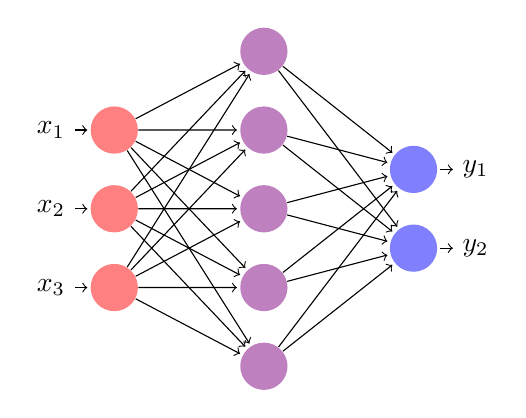
\begin{tikzpicture}

% Input Layer
\foreach \i in {1,...,\inputnum}
{
  \node[circle, 
    minimum size = 6mm,
    fill=red!50] (Input-\i) at (0,-\i) {};
}

% Hidden Layer
\foreach \i in {1,...,\hiddennum}
{
  \node[circle, 
    minimum size = 6mm,
    fill=violet!50,
    yshift=(\hiddennum-\inputnum)*5 mm
  ] (Hidden-\i) at (1.9,-\i) {};
}

% Output Layer
\foreach \i in {1,...,\outputnum}
{
  \node[circle, 
    minimum size = 6mm,
    fill=blue!50,
    yshift=(\outputnum-\inputnum)*5 mm
  ] (Output-\i) at (3.8,-\i) {};
}

% Connect neurons In-Hidden
\foreach \i in {1,...,\inputnum}
{
  \foreach \j in {1,...,\hiddennum}
  {
    \draw[->, shorten >=1pt] (Input-\i) -- (Hidden-\j);	
  }
}

% Connect neurons Hidden-Out
\foreach \i in {1,...,\hiddennum}
{
  \foreach \j in {1,...,\outputnum}
  {
    \draw[->, shorten >=1pt] (Hidden-\i) -- (Output-\j);
  }
}

% Inputs
\foreach \i in {1,...,\inputnum}
{            
  \draw[<-, shorten <=1pt] (Input-\i) -- ++(-0.5,0)
    node[left]{$x_{\i}$};
}

% Outputs
\foreach \i in {1,...,\outputnum}
{            
  \draw[->, shorten <=1pt] (Output-\i) -- ++(0.5,0)
    node[right]{$y_{\i}$};
}

\end{tikzpicture}

  \vspace{-0.8cm}
  \caption{Et simpelt neuralt netværk}
  \label{fig:neural_network}
  \vspace{0.5cm}
  \includegraphics[width=6cm]{mnist1.jpg}
  \vspace{-0.8cm}
  \caption{Eksempel fra MNIST datasættet \parencite{LeCun_1994}}
  \label{fig:mnist}
\end{wrapfigure}
Et neuralt netværk er en matematisk model, der er inspireret af de biologiske neuroner i menneskehjernen. Et neuralt netværk består af en række lag, hvor hvert lag består af neuroner. Dette kan ses på \figureref{fig:neural_network}. Hvert neuron i et lag er forbundet til alle neuroner i det forrige lag og det næste lag. Hver forbindelse mellem neuronerne har en vægt, der bestemmer, hvor meget signalet fra det ene neuron påvirker det næste neuron. Hvert neuron har også en bias, der bestemmer, hvor let det er for neuronet at sende et signal. Et neuralt netværk består af et \color{red!90}inputlag\color{black}, et eller flere \color{violet!90}skjulte lag \color{black} og et \color{blue!90}outputlag\color{black}. Dette er illustreret på \figureref{fig:neural_network}. Det er altså denne model, der er inspireret af de mange sammenkoblede neuroner i menneskehjernen. Denne lighed er ikke tilfældig, da neurale netværk er designet til at efterligne hjernens evne til at lære.\\
Bemærk \figureref{fig:mnist}. Du ved udmærket godt, hvilke tal der er på billedet, selvom du aldrig før har set netop dette 5-, 7- og 8-tal før. Dette er, fordi din hjerne er trænet til at genkende tal. Denne opgave er enormt udfordrende for et alment computerprogram, idet det ikke har nogen intuitiv forståelse af, hvad et tal er, og det skal derfor programmeres med specifikke instruktioner for at kunne genkende tal. Denne tilgang er ikke optimal, da den kræver, at programmøren har en dyb forståelse af, hvordan tal ser ud, og hvordan de kan genkendes. Denne metode er ikke holdbar i længden, idet der er uendeligt mange måder at skrive et 7-tal på. For at kunne generalisere talgenkendelse og gøre metoden mere robust overfor nye skrivemåder af tal kan neurale netværk anvendes. Antag et neuralt netværk med et tal som input og de helt rigtige vægte og biases. Denne model vil i teorien kunne genkende tal, også selvom modellen aldrig før har set netop dette tal. Håbet er, at modellen har "lært" at generalisere træningsdataen til en mere generel forståelse af tal. Modellens output vil derfor være en søjlevektor med sandsynligheder for, at inputtet er et tal fra 0 til 9. Modellens prediktering vil være det tal, der har den højeste sandsynlighed ifølge modellen.
\clearpage
\subsubsection{Feedforward}
Når modellen skal prediktere, altså gå fra input til output, kaldes dette for \textit{feedforward}. Her sendes inputtet gennem alle lagene i modellen, og bliver bliver påvirket af vægtene mellem neuronerne og biaset i hvert neuron. Herunder er et simpelt neuralt netværk med kun 1 neuron i hvert lag og et skjult lag og hvor $a_n$ er aktiveringen af neuronen i lag $n$ og $w_n$ er vægten mellem neuronen i lag $n$ og lag $n+1$:
\begin{center}
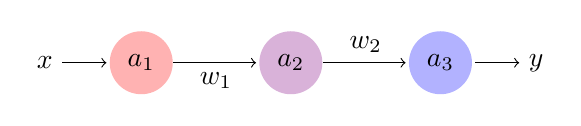
\begin{tikzpicture}
  \node[circle, minimum size=8mm, fill=red!30] (Input-1) at (0,0) {$a_1$};  % Input Layer
  \node[circle, minimum size=8mm, fill=violet!30] (Hidden-1) at (1.9,0) {$a_2$};  % Hidden Layer
  \node[circle, minimum size=8mm, fill=blue!30] (Output-1) at (3.8,0) {$a_3$};  % Output Layer
  \draw[->, shorten >=1pt] (Input-1) -- (Hidden-1) node[midway, below]{$w_1$};  % Connect neurons
  \draw[->, shorten >=1pt] (Hidden-1) -- (Output-1) node[midway, above]{$w_2$};  % Connect neurons
  \draw[<-, shorten <=1pt] (Input-1) -- ++(-1,0) node[left]{$x$};  % Inputs
  \draw[->, shorten <=1pt] (Output-1) -- ++(1,0) node[right]{$y$};  % Outputs
\end{tikzpicture}
\captionof{figure}{Et simpelt neuralt netværk}
\label{fig:neural_network2}
\end{center}
Så hvis vi ønsker at prediktere outputtet $y$ givet inputtet $x$, så kan vi gøre dette ved at følge disse trin: \\
\begin{align}
a_1 &= x
\\
a_2 &= \sigma(w_1 \cdot a_1 + b_1)
\\
a_3 &= \sigma(w_2 \cdot a_2 + b_2)
\\
y &= a_3
\end{align}
Her er $\sigma(x)$ en aktiveringsfunktion, der tager inputtet $x$ og returnerer et output. Denne funktion er essentiel for at modellen kan lære mere komplekse femomener, da den introducerer ikke-linearitet i modellen. En af de mest brugte aktiveringsfunktioner er ReLU, der tager inputtet $x$ og returnerer $x$ hvis $x > 0$ og 0 ellers. \parencite{Sanderson_2017} Hvis outputtet skal betragtes som en sandsynlighed, er sigmoid funktionen en god aktiveringsfunktion, da den tager inputtet $x$ og returnerer en værdi mellem 0 og 1, som kan tolkes som en sandsynlighed. Sigmoid funktionens definition samt et plot af funktionen er vist herunder: \parencite{Nielsen_2019a}\\
\begin{minipage}{0.4\textwidth}
  \begin{align}
    \sigma(x) = \frac{1}{1 + e^{-x}}
  \end{align}
\end{minipage}
\begin{minipage}{0.6\textwidth}
  \begin{center}
    \begin{tikzpicture}
      \draw[->] (-3,0) -- (3,0) node[right]{$x$};
      \draw[->] (0,-0.5) -- (0,1.5) node[above]{$\sigma(x)$};
      \foreach \x in {-3,-2,-1,1,2,3}
        \draw (\x,0.05) -- (\x,-0.05) node[below] {\x};
      \foreach \y in {1}
        \draw (0.05,\y) -- (-0.05,\y) node[left] {\y};
      \draw[domain=-3:3,smooth,variable=\x,red] plot ({\x},{1/(1 + exp(-\x))});
    \end{tikzpicture}
    \captionof{figure}{Sigmoid funktionen}
    \label{fig:sigmoid}
  \end{center}
\end{minipage}
Typisk har et neuralt netværk flere neuroner i hvert lag, og antallet af vægte og biases er derfor meget større. $x$, $y$, samt alle de forskellige $a_n$ og $b_n$ for hvert lag er søjlevektorer, og $w_n$ i alle lag er matricer. og derfor skal der bruges matrixmultiplikation for at kunne beregne outputtet. Dette er ikke et problem, da de pågældende regneoperationer er defineret tidligere i afsnittet.  

\subsubsection{Træning af neurale netværk}
Når et neuralt netværk initialiseres, er alle vægtene og biases tilfældige. \parencite{Sanderson_2017} Dette betyder, at modellen ikke kan genkende noget, ligesom et barn, der skal lære noget for første gang. For at lære modellen at genkende tal, skal modellen trænes. Dette kræver en anstændig mængde træningsdata og associerede labels, der fortæller modellen, hvad hvert billede er. For at træne modellen skal man vide hvor god modellen er til at prediktere datasættet, en primitiv måde at gøre det på er at angive procenten af rigtigt predikterede tal. Denne metode er ikke velfungerende, da en lille ændring i vægtene og biases vil ændre modellens præstation minimalt og er derfor ikke målbar. For at kunne træne modellen effekt skal vi vide præcist hvordan en lille ændring i vægtene og biases påvirker modellens præstation. Denne funktion kaldes en \textit{loss funktion}, og er essential for at kunne træne modellen. Loss funktionen er en funktion, der tager modellens prediktion og sammenligner den med det rigtige svar. Loss funktionen er en måde at kvantificere, hvor god modellen er til at prediktere. Hvis loss funktionen er høj, er modellen dårlig til at prediktere, og hvis loss funktionen er lav, er modellen god til at prediktere. herunder ses et eksempel på en loss funktion på et enkelt datapunkt $i$ \parencite{Sanderson_2017}:
\begin{wrapfigure}[5]{r}{4cm}
  \includegraphics[width=4cm]{mnist2.jpg}
  \vspace{-0.8cm}
  \caption{Eksempel på et 2-tal fra MNIST datasættet \parencite{LeCun_1994}}
  \label{fig:mnist2}
\end{wrapfigure}
\begin{align}
  \underbrace{\hat{y}_i = \begin{bmatrix}
    0.12 \\
    0.03 \\
    0.25 \\
    0.07 \\
    0.18 \\
    0.09 \\
    0.04 \\
    0.11 \\
    0.06 \\
    0.05
  \end{bmatrix}}_{\text{Modellens prediktion}}
  &&
  \underbrace{y_i = \begin{bmatrix}
    0 \\
    0 \\
    1 \\
    0 \\
    0 \\
    0 \\
    0 \\
    0 \\
    0 \\
    0
  \end{bmatrix}}_{\text{Det rigtige svar}}
\end{align}
Loss funktionen for dette datapunkt er den kvadrerede forskel mellem modellens prediktion og det rigtige svar:
\begin{align}
  L_i = (y_i - \hat{y}_i)^2 = \begin{bmatrix}
    0 - 0.12 \\
    0 - 0.03 \\
    1 - 0.25 \\
    \vdots \\
    0 - 0.05
  \end{bmatrix}^2 = \begin{bmatrix}
    -0.12^2 \\
    -0.03^2 \\
    0.75^2 \\
    \vdots \\
    -0.05^2
  \end{bmatrix}
\end{align}
Nu tages summen af den kvadrerede forskel for at få loss funktionen for dette datapunkt:
\begin{align}
  L_i &= \sum_{i=1}^{10} (y_i - \hat{y}_i)^2\\
      &= (-0.12^2) + (-0.03^2) + (0.75^2) + \ldots + (-0.05^2)
\end{align}
Denne operation gentages for alle datapunkter i træningssættet, og summen tages, derefter divideres summen med antallet af datapunkter for at få gennemsnittet af loss funktionen for hele træningssættet \parencite{Sanderson_2017}:
\begin{align}
  L = \frac{1}{N} \sum_{i=1}^{N} \sum_{j=1}^{10} (y_{ij} - \hat{y}_{ij})^2
\end{align}
Nu har vi en loss funktion, der kvantificerer, hvor god modellen er til at prediktere, og hvor selv en lille ændring i vægtene og biases vil ændre loss funktionen. Nu er det muligt at træne modellen ved at minimere loss funktionen, da man kan sige at når loss funktionen er lav, er modellen god til at prediktere. Desuden er denne loss funktion kontinuert og differentiabel, hvilket er essentielt for at kunne træne modellen. For at minimere loss funktionen bruges en algoritme kaldet \textit{gradient descent}. 

\subsection{Gradient descent}
Gradient descent er en algoritme, der tager loss funktionen og beregner gradienten af loss funktionen i forhold til alle modellens parameter (vægtene og biases). Gradienten er en vektor, der peger i retningen af den største stigning af loss funktionen. For at minimere loss funktionen skal vi derfor gå i den modsatte retning af gradienten. Dette gøres ved at opdatere vægtene og biases i modellen med gradienten ganget med en konstant, kaldet \textit{learning rate}. Dette gentages indtil loss funktionen er minimeret tilstrækkeligt. \parencite{IBM_2021,Sanderson_2017,Nielsen_2019a}\\
Antag at vi organiserer modellens vægte og biases i en søjlevektor $\vec{W}$ og at loss funktionen er $L(\vec{W})$. Gradienten af loss funktionen er $\nabla L(\vec{W})$, derfor beskriver søjlevektoren $-\nabla L(\vec{W})$ hvordan vi kan opdatere $\vec{W}$ for at minimere loss funktionen og dermed øge modellens præstation. Algorimen som finder gradienten på baggrund af modelles parametre og loss funktionen kaldes \textit{backpropagation}. \parencite{Sanderson_2017,Nielsen_2019a} Det vil ses nærmere på, hvordan backpropagation fungerer i et kommende afsnit. Indtil videre antager vi blot, at den fungerer som påstået og returnerer det passende gradient for modellens parametre.

\subsection{Differensiabilitet}

\newpage
\printbibliography


\end{document}
